
\chapter{Geodesia}


\section{Definiciones básicas}

Como sabemos la tierra tiene una forma de una esfera achatada, tomando la forma de un elipsoide de revolución. En palabras de Isaac Newton: <<Una forma de equilibrio que tiene una masa bajo el influjo de las leyes de gravitación y girando en torno a su eje es la de un esferoide aplastado en sus polos>>. Un \textit{esferoide aplastado en sus polos} es básicamente un elipsoide de revolución. Definimos pues:



\begin{itemize}
	\begin{minipage}{.45\textwidth}
	\item   \textbf{Polos:} puntos de corte entre el eje menor de la elipse y elipsoide. Llamamos polo norte (PN) al corte superior y polo sur (PS) al corte superior.   
	\item \textbf{Ecuador terrestre:} línea circular correspondiente al corte entre el plano perpendicular al eje menor que pasa por el centro del elipsoide y este.
	\end{minipage}	\hfill
	\begin{minipage}{0.45\textwidth} \centering
	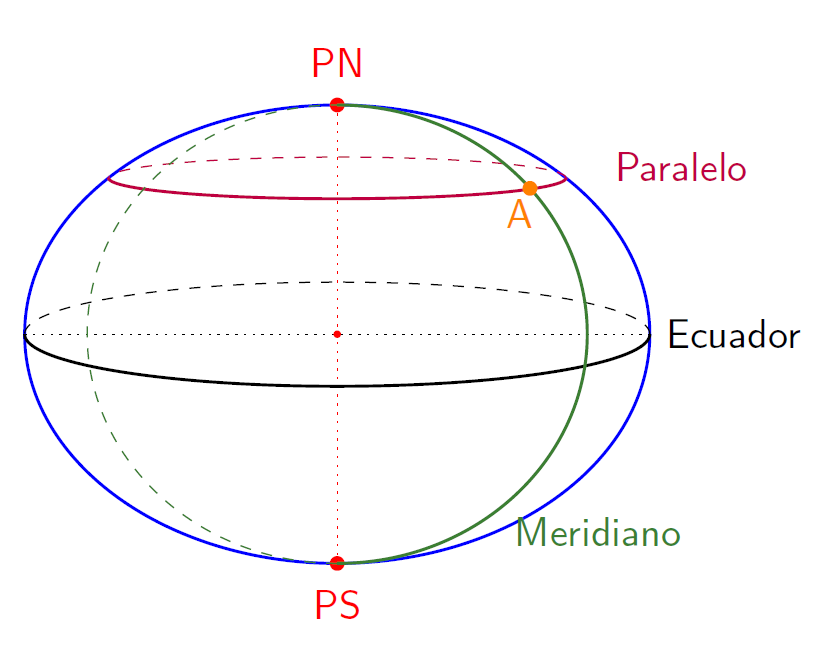
\includegraphics[scale=0.37]{Cuerpo/Imagenes/01_Elipsoide.png} 
	\end{minipage}
\end{itemize}
\begin{itemize}
	\item \textbf{Paralelos:} líneas circulares correspondientes a los cortes entre los planos paralelos al ecuador (paralelo cero) y el elipsoide.
	\item \textbf{Meridianos:} líneas elipsoidales determinadas por el corte entre el elipsoide y el hazde planos que define el eje menor. Se considera \textit{meridiano cero} al que pasa por Greenwich.
	\item \textbf{Vertical de lugar:} es la línea normal al elipsoide en un punto dado.
\end{itemize}


Al conjunto de variables que permiten describir cualquier punto de la Tierra se le llaman \textit{coordenadas terrestres}, y existen dos tipos de coordenadas terrestres, que se definen en función de la \textit{vertical de lugar}

\begin{itemize}
	\item \textbf{Coordenadas geográficas:} son dos variables angulares ($\phi,\lambda$), que se definen como

	\begin{itemize}	
		\item \textbf{Latitud geográfica} $\phi$. Toma valores de $90^\circ$ a $-90^\circ$. Para un punto $A$ cualquiera el ángulo $\phi$ es el comprendido entre la vertical de lugar y el ecuador.
		\item \textbf{Longitud geográfica} $\lambda$. Toma valores entre $180^\circ$ y $-180^\circ$. Para un punto $A$ cualquiera el ángulo $\lambda$ se define como aquel entre la vertical de lugar y el meridiano de Greenwich. 
	\end{itemize}
	
	\item \textbf{Coordenadas geocéntricas}: consta de tres variables $(\rho,\psi,\lambda)$, dos angulares y una distancia. Estas son: 
	
	\vspace{2mm}
		
	\begin{minipage}{1\textwidth}
	 \begin{itemize}
	\item \textbf{Radio vector} $\rho$. Distancia entre el centro de la tierra (punto 0) y el punto A. 
	\end{itemize}
	\end{minipage}	

	\begin{minipage}{.5\textwidth}
	\begin{itemize}
		\item \textbf{Latitud geocéntrica} $\psi$. Toma valores de $90^\circ$ a $-90^\circ$. Para un punto $A$ cualquiera el ángulo $\psi$ es el comprendido entre el radio y el ecuador. 
		\item \textbf{Longitud geocéntrica} $\lambda$. Se define igual que la longitud geográfica. Toma valores entre $180^\circ$ y $-180^\circ$. Para un punto $A$ cualquiera el ángulo $\lambda$ se define como aquel entre la vertical de lugar y el meridiano de Greenwich.
	\end{itemize}
	\end{minipage}	\hfill
	\begin{minipage}{0.5\textwidth} \centering
		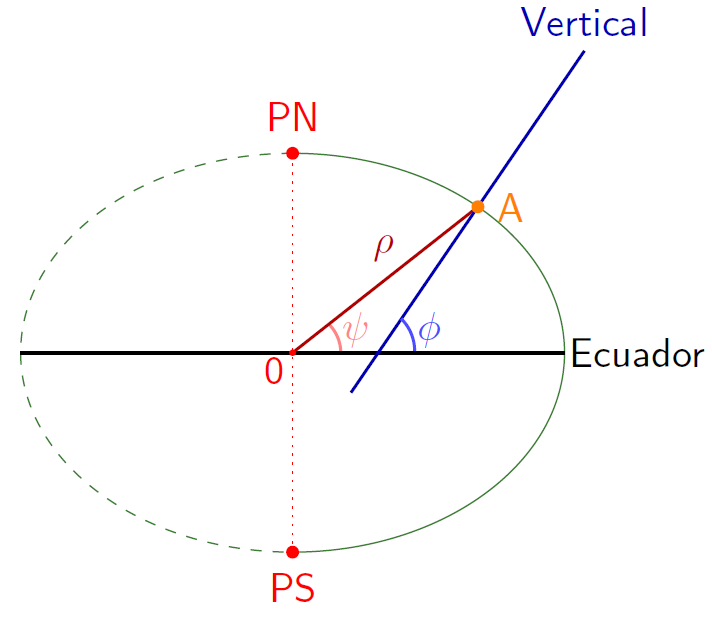
\includegraphics[scale=0.42]{Cuerpo/Imagenes/01_Coordenadas.png} 
	\end{minipage}	
	
\end{itemize}

Otra definición importante es la del \textbf{plano del horizonte}, que es el plano perpendicular a la vertical de lugar en el punto $A$. El plano horizonte pertenece a la llamada \textbf{esfera celeste topocéntrica}, que es aquella cuyo centro es el observador. En esta esfera, el plano horizonte define lo que una persona diría que es arriba y abajo. La esfera celeste tropocéntrica tiene también un polo norte celeste (PNC) y un polo sur celeste (PSC) paralelo con el eje del mundo, pero no necesariamente con el <<arriba>> del observador. Al punto $Z$ se le llama \textbf{cénit} y al punto $Z'$ se le llama \textbf{nádir}.

\begin{figure}[h]
	\centering
	\begin{subfigure}{0.55\textwidth}
		\centering
		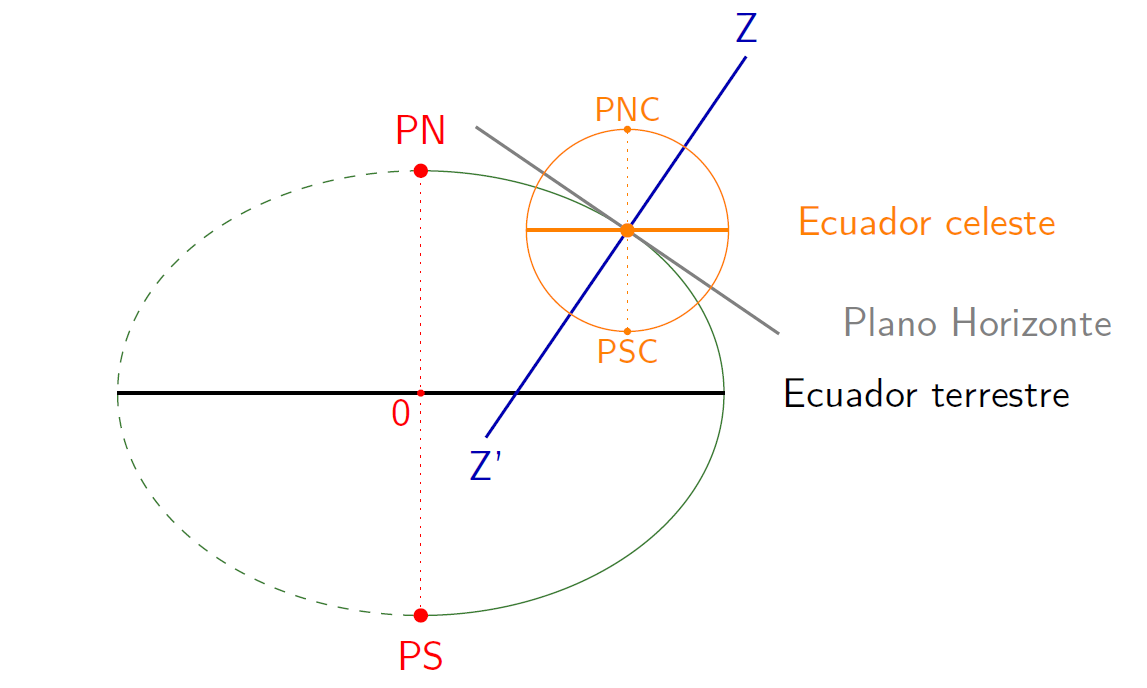
\includegraphics[width=0.9\textwidth]{Cuerpo/Imagenes/01_Plano.png}
	\end{subfigure}
	\hfill
	\begin{subfigure}{0.4\textwidth}
		\centering
		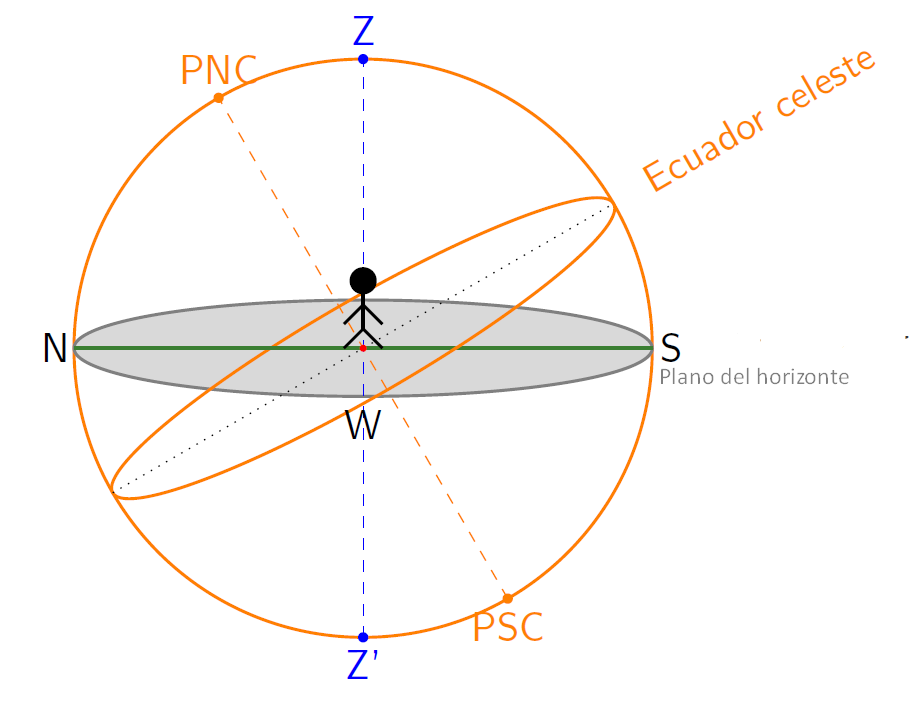
\includegraphics[width=0.9\textwidth]{Cuerpo/Imagenes/01_Esfera.png}
	\end{subfigure}
\end{figure}
Como podemos ver el ángulo entre la línea PNC y Z en la esfera topocéntrica es igual a $90^\circ - \phi$, y por tanto independiente al meridiano en el que nos encontremos, solo depende del paralelo en el que se encuentre el punto del observador. A dicho ángulo se le llama \textbf{colatitud}.

\hspace{-6.0mm}
\begin{minipage}{0.6\textwidth}
El \textbf{plano de la eclíptica} es el plano que contiene la órbita de la Tierra alrededor del Sol, y está inclinado con respecto al ecuador celeste una cantidad llamada \textit{oblicuidad de la eclíptica} $\varepsilon=20^\circ 26'29''$. En la esfera celeste geocéntrica, cuyo centro es la Tierra, es el Sol quien aparenta moverse a nuestro alrededor. Llamamos \textbf{eclíptica} a la intersección del plano de la eclíptica con la esfera celesta. % 
\end{minipage}	\hfill
\begin{minipage}{0.4\textwidth} \centering
		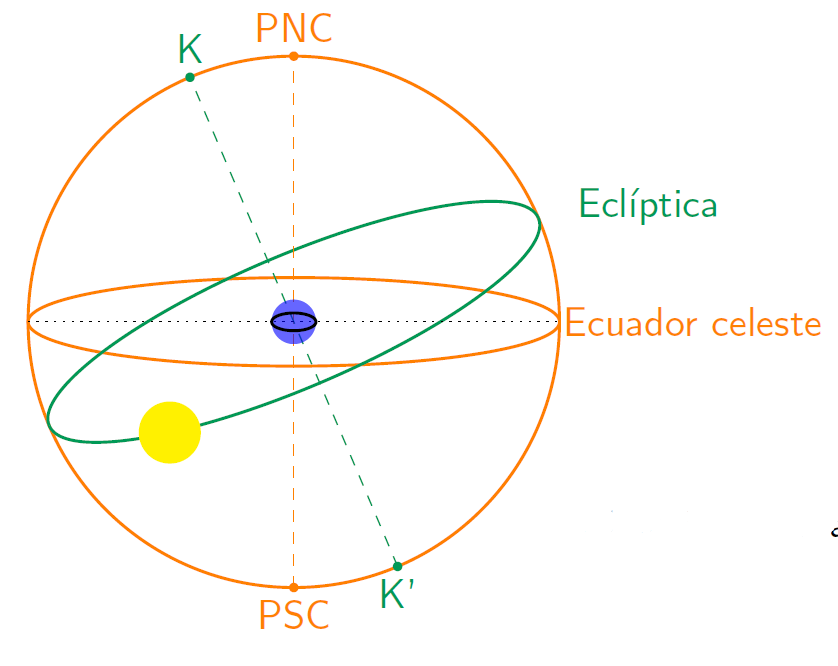
\includegraphics[width=0.8\textwidth]{Cuerpo/Imagenes/01_Ecliptica.png}	
\end{minipage}	


%El \textbf{plano de la eclíptica} es el plano que contiene la órbita de la Tierra alrededor del Sol, y está inclinado con respecto al ecuador celeste una cantidad llamada \textit{oblicuidad de la eclíptica} $\varepsilon=20^\circ 26'29''$. En la esfera celeste geocéntrica, cuyo centro es la Tierra, es el Sol quien aparenta moverse a nuestro alrededor. Llamamos \textbf{eclíptica} a la intersección del plano de la eclíptica con la esfera celesta.

\section{Coordenadas astronómicas}

Las coordenadas astronómicas nos sirven para designar la posición de un astro en la bóveda celeste. Todos los sistemas de coordenadas que se usan en astronomía son sistemas esféricos/polares, designando cualquier punto de la esfera celeste con dos ángulos. Toda diferencia entre dos sistemas de coordenadas distintos radica en 4 puntos: la definición de lo que llamamos \textit{plano fundamental}, su \textit{eje x}, \textit{el centro de la esfera elegido}, y si el sistema de coordenadas es \textit{dextrógiro} o \textit{levógiro}. Así, tenemos dos clasificaciones:

\begin{itemize}
	\item En función del centro de la esfera: \begin{itemize}
		\item \textbf{Topocéntrico:} el centro es el observador.
		\item \textbf{Geocéntrico:} el centro es la tierra.
		\item \textbf{Helicéntrico:} el centro es el sol.
	\end{itemize}
	\item En función del plano fundamental: \begin{itemize}
	\item \textbf{Horizontales:} en este caso el plano fundamental es el {plano del hoirzonte.}.
	\item \textbf{Ecuatoriales:} el plano ecuatorial es el plano fundamental.
	\item \textbf{Eclíptica:} el plano de la eclíptica es el plano fundamental.
	\end{itemize}
\end{itemize}
Un sistema es \textbf{levógiro} cuando el ángulo azimutal (el que manda en el plano fundamental) sigue el sentido antihorario mirando en el sentido del eje X, mientras que es \textbf{dextrógiro} si sigue en el sentido horario. La definición del eje X depende del sistema, y será definida en cada apartado. 

\subsection{Coordenadas Horizontales}

Las coordenadas horizontales usan el horizonte como plano fundamental, es un tipo de sistema levógiro y el eje X para cualquier observador es aquel que apunta al sur (hemisferio norte) o que apunta al norte (hemisferio sur). Las coordenadas son:

\begin{itemize}
	\item La \textbf{altura} $h$. Tiene valores desde los $90^\circ$ a $-90^\circ$ Para un punto de la esfera celeste, se define como el ángulo entre el plano horizonte y la línea que conecta el observador y el punto. La \textit{distancia cenital} se define como el ángulo entre el vector normal del plano y la línea que conecta el observador y el punto.
	\item El \textbf{acimut} $A$ se define como el ángulo entre el eje X y la proyección en el plano fundamental del la línea que conecta el observador y el punto, creciendo en el sentido levógiro. 
\end{itemize}

\begin{figure}[h]
	\centering
	\begin{subfigure}{0.45\textwidth}
		\centering
		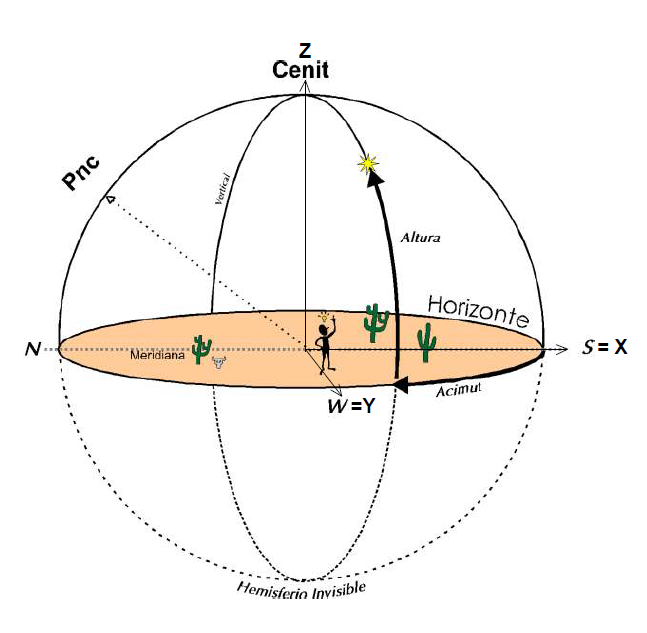
\includegraphics[width=0.8\textwidth]{Cuerpo/Imagenes/01_Horizontales.png}	
		\caption{Coordenadas horizontales.}
	\end{subfigure}
	\hfill
	\begin{subfigure}{0.45\textwidth}
		\centering
		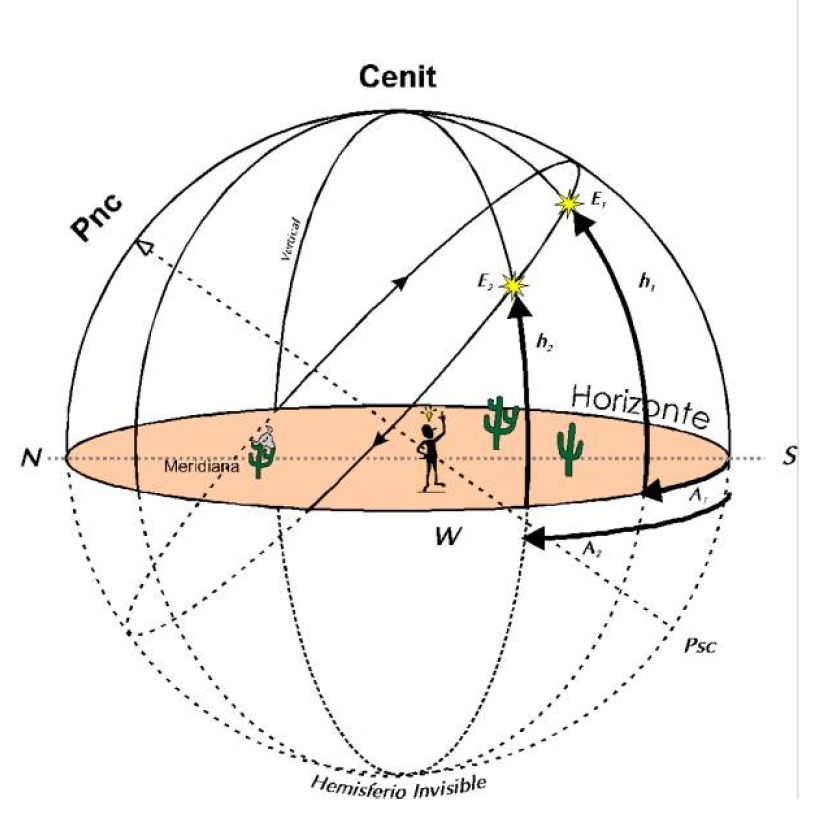
\includegraphics[width=0.75\textwidth]{Cuerpo/Imagenes/01_Horizontales_2.png}	
		\caption{Cambio de posición del sol a lo largo del día.}
	\end{subfigure}
\end{figure}

\newpage

Este sistema es un sistema local, es decir, los astros dependen del lugar del punto en la tierra desde el que se está observando. Además, también varían en función del momento del día. Esto es evidente si pensamos por ejemplo en el sol: para diferentes horas del día se encontrará a diferente altura (y en diferente acimutal). 

\subsection{Coordenadas ecuatoriales horarias}

En este sistema el plano fundamental es el ecuador celeste, siendo el eje $z$ entonces el eje del mundo. Es un sistema levógiro, que define el eje X como aquel que apunta hacia el sur (hemisferio norte) o que apunta hacia el norte (hemisferio sur), pero que se encuentra en el plano ecuador. Las coordenadas son:

\hspace{-8.0mm} \vspace{1.0mm} \begin{minipage}{0.6\textwidth}
\begin{itemize}
	\item La \textbf{declinación} $\delta$, definida igual que la altura para las coordenadas horizontales pero ahora usando como referencia el plano ecuatorial.  Tiene valores desde los $90^\circ$ a $-90^\circ$ Para un punto de la esfera celeste, se define como el ángulo entre el plano ecuatorial y la línea que conecta el observador y el punto. La diferencia entre la altura y la declinación dependerá del paralelo en la que nos encontremos. 
	\item Definimos el \textbf{ángulo horario} $H$ como el acimut, el ángulo entre el eje $x$ y la proyección en el plano ecuatorial de la línea que conecta en observador y el punto, en un sentido levógiro. 
\end{itemize}
\end{minipage}	\hfill
\begin{minipage}{0.35\textwidth} \centering
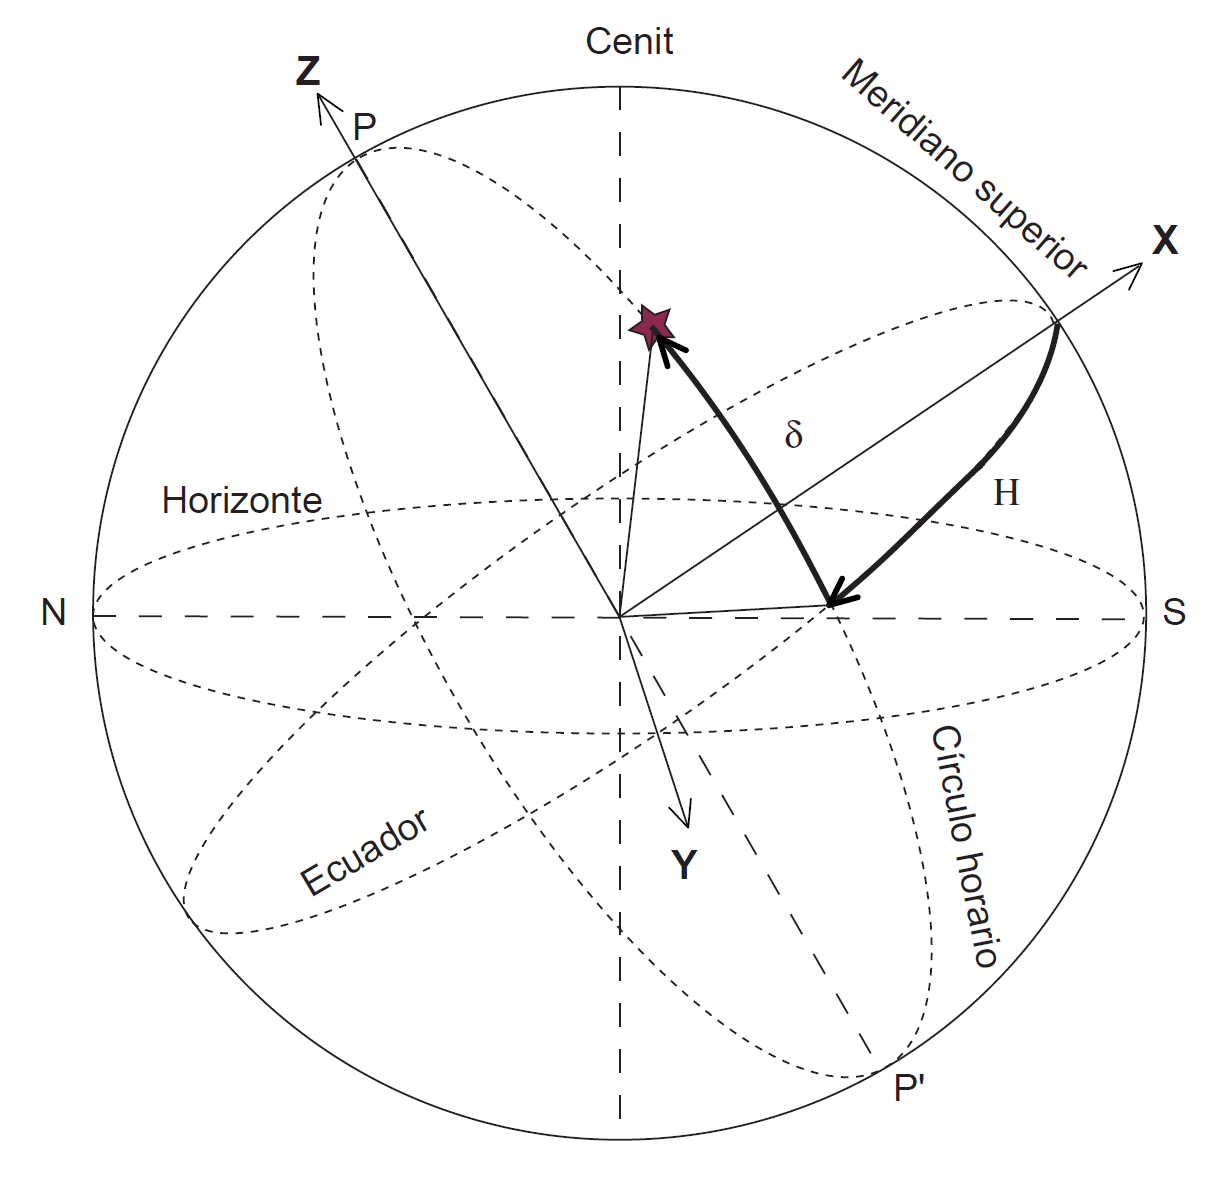
\includegraphics[width=1\textwidth]{Cuerpo/Imagenes/01_Ecuatoriales_Horarias.png}	
\end{minipage}	

\subsection{Coordenadas ecuatoriales absolutas}

En este sistema el plano fundamental es el ecuador celeste, siendo el eje $z$ entonces el eje del mundo. Es un sistema dextrógiro, que define el eje X como aquella recta del plano ecuatorial que se interseca con la eclíptica. También se le llama \textit{línea del equinocio}. Recordemos que el equinocio es auqel momento del año en el que el plano ecuatorial y el plano eclíptico coinciden, mientras que el solsticio aquel en el que el ángulo entre ambos es máximo (eclíptica $\varepsilon$). pero que se encuentra en el plano ecuador. Las coordenadas son:

\hspace{-8.0mm} \vspace{1.0mm} \begin{minipage}{0.6\textwidth}
\begin{itemize}
	\item La \textbf{declinación} $\delta$, definida igual que en el sistema ecuatorial horario, tiene valores desde los $90^\circ$ a $-90^\circ$ Para un punto de la esfera celeste, se define como el ángulo entre el plano ecuatorial y la línea que conecta el observador y el punto. La diferencia entre la altura y la declinación dependerá del paralelo en la que nos encontremos. 
	\item Definimos el \textbf{ascensión recta} $\alpha$ como el acimut, el ángulo entre el eje $x$ y la proyección en el plano ecuatorial de la línea que conecta en observador y el punto, en un sentido levógiro. 
\end{itemize}
\end{minipage}	\hfill
\begin{minipage}{0.35\textwidth} \centering
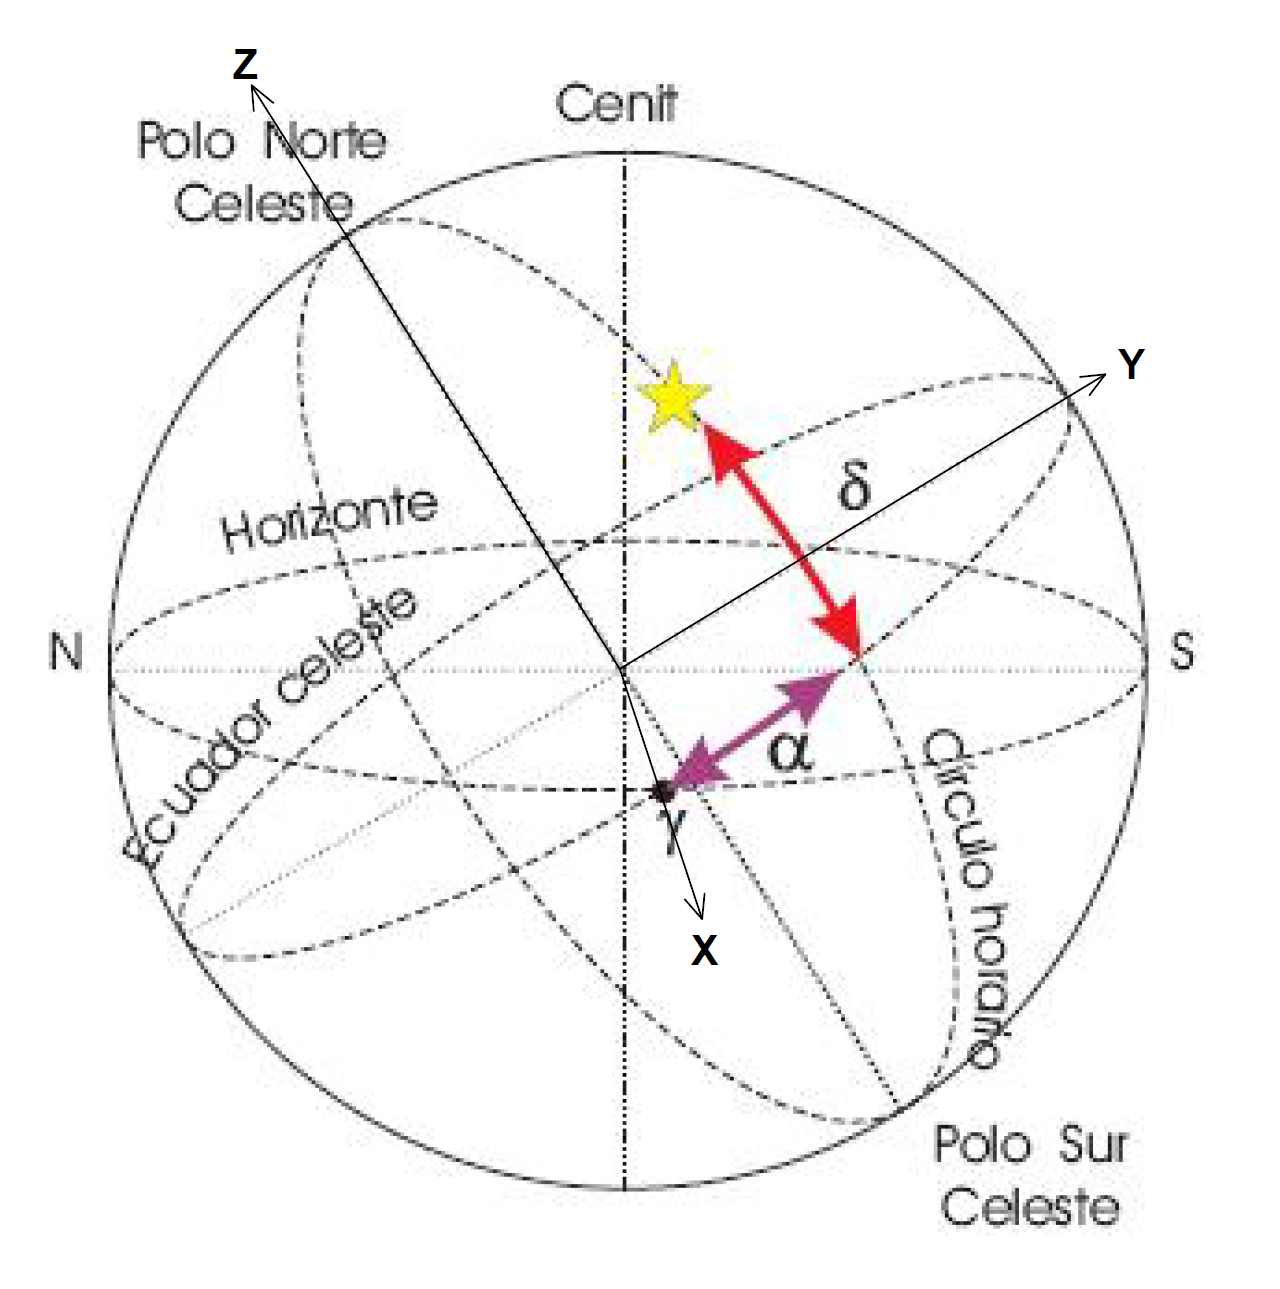
\includegraphics[width=1\textwidth]{Cuerpo/Imagenes/01_Ecuatoriales_Absolutas.png}	
\end{minipage}	



\subsection{Coordenadas eclípticas}

Las coordenadas eclípticas $(\lambda,\beta)$ son exactamente iguales que las coordendas ecuatorilaes absolutas pero usando el plano eclíptico como plano fundamental. El eje $x$ entre ambos es el mismo, por lo que la única diferencia entre ambos sistemas es una rotación $\varepsilon$ (ángulo entre el plano eclíptico y el plano ecuatorial).

\begin{Anotacion}
	\textcolor{red}{Aquí tenemos que hablar de las coordenadas horizontales y horarias de la esfera celeste. Para que sirven cada una, como se definen. Relaciones entre ellas.}
\end{Anotacion}	



\begin{Anotacion}
	\textcolor{red}{Esfera celeste, en este orden: coordenadas eclípticas, horizontales, absolutas. Para que sirve cada uno, cuales son los ángulos de referencia. En las ecuatoriales hay que hablar de los ángulos del equinocio y solscitio del sol. En lass horizontales también. Como se cambia de un sistema de coordenadas a otra. Matrices de rotación. Tiempo sideral. Diferencia entre levógiro y dextrógiro. }
\end{Anotacion}	

%Las coordenadas celestes ecuatoriales absolutas y eclípticas constituyen sistemas de coordenadas absolutos, siendo independientes de los movimientos de rotación y traslación de la Tierra. Sin embargo, existen otros movimientos de la Tierra que sí afectan a las coordenadas. Veremos los movimietnos de precesión y nutación. 

\section{Ejercicios}


\tcbstartrecording
\begin{texercise}
	
	Prueba que el azimut y el ángulo horario de un astro en sus puntos de orto y ocaso, $A_0$ y $H_0$, para un observador a una latitud $\phi$, satisfacen la siguientes relaciones:
	
	\begin{equation}
		\cos (A_0) = - \frac{\sin (\delta)}{\cos (\phi)} \tquad \cos (H_0) = - \tan \delta \tan \phi
	\end{equation}
	\tcblower

	Recordamos que el orto y ocaso son los lugares del plano horizonte donde empieza a ser visible y deja de ser visible. Con respecto las coordenadas horizontales, la altura es cero $h=0^\circ$, o lo que es lo mismo $z=90^\circ$. Ahora tenemos que usar las coordenadas de Bessel, que relaciona las coordenadas horizonatles (A,h) y horarias ($H,\delta$):
	
	\begin{equation}
	\begin{pmatrix}
		\cos \delta \cos H \\
		\cos \delta \sin H \\
		\sin \delta 
	\end{pmatrix} =\begin{pmatrix}
		\sin \phi & 0 & \cos \phi \\
		0 & 1 & 0 \\
		- \cos \phi & 0 & \sin \phi
	\end{pmatrix}
	\begin{pmatrix}
		\cos h \cos A \\
		\cos h \sin A \\
		\sin h
	\end{pmatrix}
	\end{equation}
	de lo cual se deduce que
	
	\begin{equation}
	\sin \delta = - \cos (\phi) \cos A_0  \Rightarrow \cos (A_0) = - \frac{\sin \delta}{\cos \phi}
	\end{equation}
	Y también se deduce que
	
	\begin{equation}
	\cos \delta \cos H_0 = \sin \phi \cos A_0 \Rightarrow \cos (H_0) = \frac{\sin \phi}{\cos \delta} \parentesis{ - \frac{\sin \delta}{\cos \phi}} \Rightarrow \cos (H_0) = - \tan \delta \tan \phi
	\end{equation}
\end{texercise}

\begin{texercise}
	 ¿Cómo relacionarías la información proporcionada por $H_0$ con el tiempo que un astro permanece por encima del horizonte?
	 \tcblower
	 
	 \begin{minipage}{.45\textwidth} 	
	 	El tiempo que un astro está encima del horizonte corresponde a $2H_0$. Puso $H_{\text{orto}}=-H_{\text{ocaso}}$.
	 \end{minipage}	\hfill
	 \begin{minipage}{0.45\textwidth} 
	 	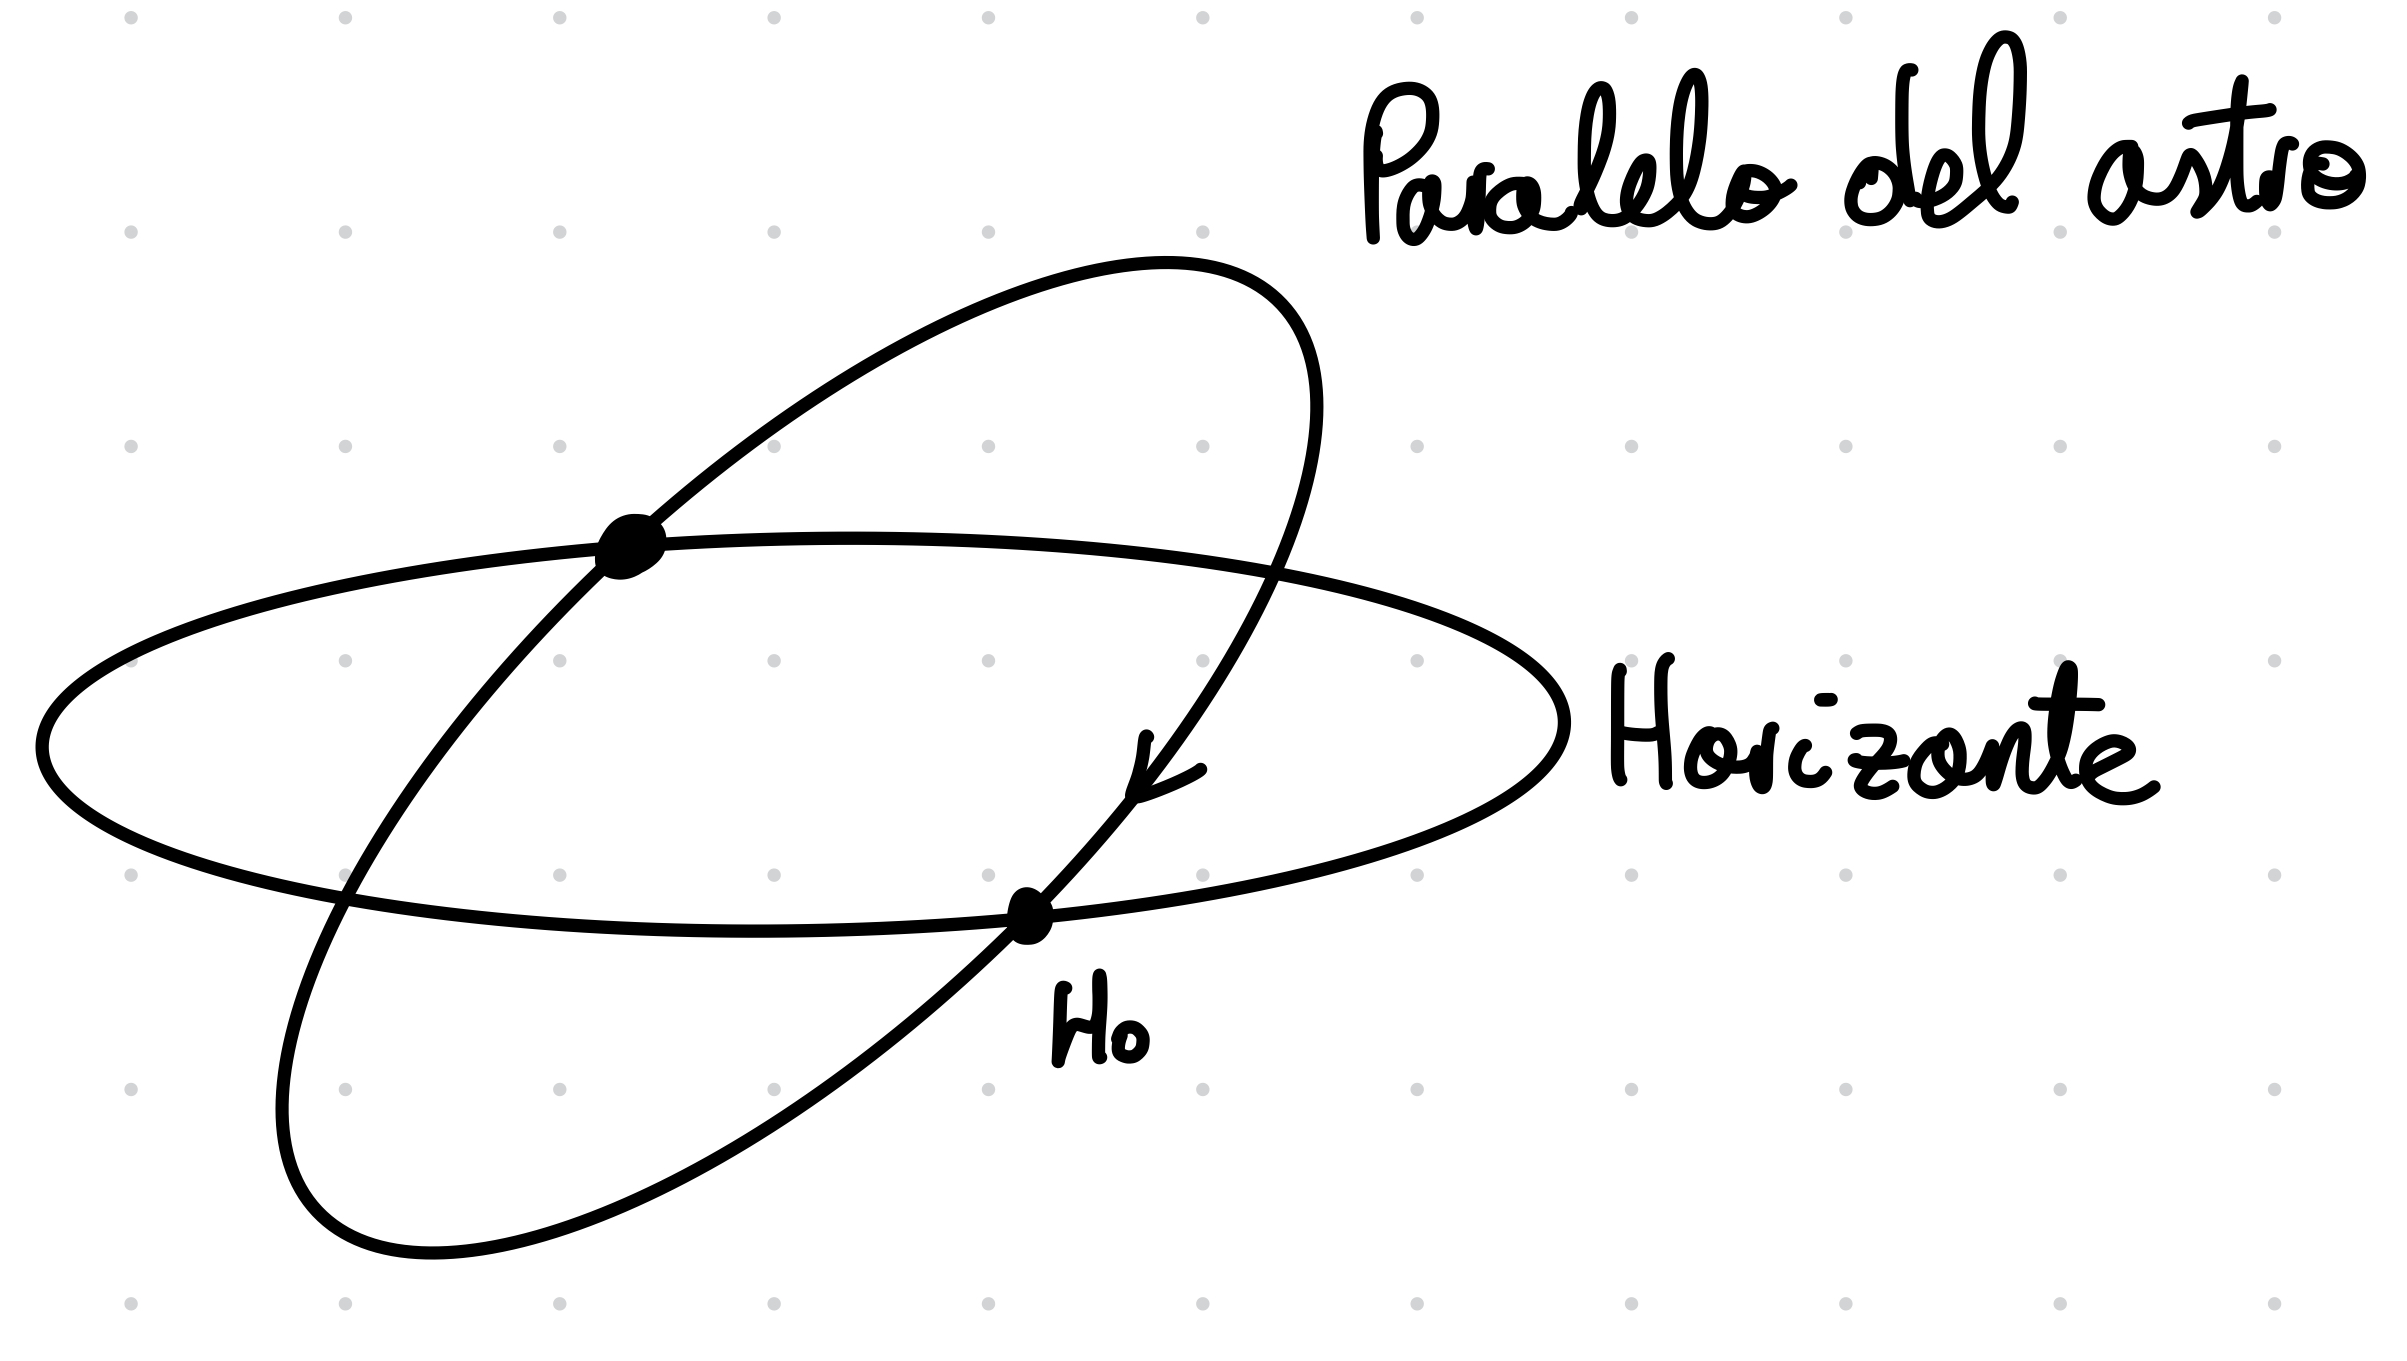
\includegraphics[width=1.0\textwidth]{Cuerpo/Imagenes/01_Ejercicio_2.jpg}
	 \end{minipage}
	 
	 
\end{texercise}

\begin{texercise}
	¿Cuántas horas máximas y mínimas del Sol por encima del horizonte a lo largo de un día podemos tener en Santiago de Compostela? Dato: $\phi=42^\circ,52',40''$.
	 \tcblower
		 
	El máximo de horas ocurre cuando estamos el solsticio de verano. En este caso sabemos que $\delta=\epsilon$. Usando las ecuaicones del primer ejercicio:
		 
	 \begin{equation}
	 	H_0 = 7^h 34^m 57^s \Rightarrow 2H_0 = 15^h 9^m 54^s
	 \end{equation}
	 El mínimo de horas del sol es en el solsticio de invierno.  En este caso
		 
	 \begin{equation}
	 	\delta = - \varepsilon \Rightarrow 2H_0 = 8^h 50^m 4^s
	 \end{equation}
\end{texercise}


\begin{texercise}
	Las coordenadas ecuatoriales absolutas de una estrella son 	$\alpha = 3^{h}45^{m}43^{s}$, y $\delta = 20^\circ8'27''$. ¿Podremos observarla desde la Facultad de Matemáticas ($\phi = 42^\circ52'26''$) en el instante en el que el punto 
	vernal está en la dirección norte? \textbf{[Solución:} Dado que $h < 0^\circ$ 
	($h = -8^\circ24'29''$), la estrella no será visible.\textbf{]}
	\tcblower
	Nos dan las coordenadas ecuatoriales absolutas. La condición para no ver un astro desde un punto de la tierra es que dicho astro, en las coordenadas horizontales, verifique que su altura tiene ángulos negativos ($h<0^\circ$). Consecuentemente solo tenemos que calcular $h$ a partir de $\alpha$ y $\delta$. ¿Cómo lo hacemos? 
	
	Primero calculamos el valor de las coordenadas ecuatoriales horarias. Como sabemos $\delta_{\mathrm{horaria}} = \delta_{\mathrm{absolutas}}$ y $\alpha+H=\theta$, siendo $\theta$ la posición del punto vernáculo en las horizontales. Cuando nos dicen que el punto vernáculo apunta al norte, nos están dado el dato de $\theta$. Como $x$ en las horarias apunta al sur, $\theta=180^\circ$. Así pues:

	\begin{equation}
		H = 12^h - 3^h 45^m 43^s = 8^h 14^m 17^s \approx 120.24^\circ  \tquad \delta=20^\circ 8'27''
	\end{equation}
	Ahora solo tenemos que transformar las coordenadas ecuatoriales horarias en las horizontales. Esto también es sencillo, ya que es rotar un $\phi$ los ejes $x$ y $z$, tal que: 
	
	\begin{equation}
		\begin{pmatrix}
			\cos h \cos A \\
			\cos h \sin A \\
			\sin h 
		\end{pmatrix} =\begin{pmatrix}
			\sin \phi & 0 &- \cos \phi \\
			0 & 1 & 0 \\
			 \cos \phi & 0 & \sin \phi
		\end{pmatrix}
		\begin{pmatrix}
			\cos \delta \cos H \\
			\cos \delta \sin H \\
			\sin \delta
		\end{pmatrix}
	\end{equation}
	Y ya podríamos obtener el valor de $h$, solo faltando despejar. Teniendo en cuenta que $\phi=42^\circ52'26''$. Para calcular $h$ (que es lo único que necesitamos en realidad) despejamos:

	\begin{equation}
		\sin h = \cos \phi \cos \delta \cos H + \sin \phi \sin \delta
	\end{equation}
	que es: 
	\begin{equation}
		\sin h = -0.1125 \quad \Longrightarrow \quad h = -6.46^\circ
	\end{equation}
	La solución correcta es $h = -8^\circ24'29''$. La diferencia es posiblemente culpa de los decimales, porque no hemos convertido correctamente los segundos y minutos. 
\end{texercise}
\begin{texercise}
	Un cometa tiene coordenadas ecuatoriales absolutas $\alpha = 10^{h}3^{m}57^{s}$ y $\delta = 8^\circ24'54''$. ¿Cuáles son sus coordenadas eclípticas?  
	\textbf{[Solución:} $\lambda = 150^\circ3'19''$	$\beta = -3^\circ14'31''$.\textbf{]}
	\tcblower
	Para pasar de las coordenadas ecuatoriales absolutas a las coordenadas eclípticas solo tenemos que hacer una rotación, ya que el eje $x$ es el mismo (punto vernal). Así pues, solo tenemos que aplicar la matriz de rotación: 

	\begin{equation}
		\begin{pmatrix}
			\cos \beta \cos \lambda \\
			\cos \beta \sin \lambda \\
			\sin \beta
		\end{pmatrix} =\begin{pmatrix}
			1 & 0 & 0 \\
			0 & \cos \epsilon & \sin \epsilon \\
			0 & -\sin \epsilon &  \cos \epsilon
		\end{pmatrix}
		\begin{pmatrix}
			\cos \delta \cos \alpha \\
			\cos \delta \sin \alpha \\
			\sin \delta
		\end{pmatrix}
	\end{equation}
	Recordamos que $\varepsilon=20^\circ 26' 29''$, $\alpha = 10^{h}3^{m}57^{s}$ y $\delta = 8^\circ24'54''$. Primero obtenemos $\beta$:

	\begin{equation}
		\sin \beta = - \sin \epsilon \cos \delta \sin \alpha + \cos \epsilon \sin \delta 
	\end{equation}
	\begin{equation}
		\sin \beta = 0.05986\quad \Longrightarrow \quad \beta = 3.432^\circ
	\end{equation}
	Luego solo tenemos que despejar $\lambda$. Sabiendo que 

	\begin{equation}
		\cos \lambda = \frac{\cos \delta \cos \alpha}{\cos \beta} \Rightarrow \cos \lambda = -0.853^\circ \Rightarrow \lambda = 150.19^\circ
	\end{equation}
	Siendo la solución correcta $\lambda = 150^\circ3'19''$	$\beta = -3^\circ14'31''$.
\end{texercise}

\tcbstoprecording
